% !TeX root = interim.tex

\iffalse


\fi

\subsection{Project Schedule}
% discuss what we are behind on/ ahead on. Mention progress reports 1&2

The updated project timeline in the form of a Gantt chart can be found in \autoref{app:gantt_chart}. So far we have been on track with our initial timeline stated in our proposal report \autocite{proposal_report}. Progress was halted closer to the end of the term due to assignment deadlines for other modules. However we plan to make up the lost time over the Christmas holiday to ensure that we will not fall behind schedule.

\subsection{Supporting Theory}

    \subsubsection{Neural Networks and Deep Learning}
        \hspace*{0pt}\hfill \textit{Oliver Jaison}\\
        
        Autoencoders are a special type of artificial neural network where, rather than the number of filters increasing in subsequent hidden layers from the input layer, we impose a bottleneck. This means that the number of filters is less than the number of inputs in the input layer. This results in a compressed representation of the input data. Traditionally this is an unsupervised learning algorithm but it is made semi-supervised by comparing the output of the autoencoder to the input and minimising the error between them.
        \\
        
        \autocite{8820761} Explains that autoencoder based compression methods in communication channels learn the statistical regularities in the data. This could be key in an error correcting system for a transmitter receiver pair with correlated input data.
        \\
        
        \autoref{fig:autoencoder} shows a very basic autencoder but similarly with neural networks you can have different categories of autoencoder. \autocite{9058605} Talks about a de-noising autoencoder. A de-noising autoencoder will corrupt the input on purpose then compare the output to the un-corrupted input to generate a loss function. This loss function is then fed back into the input to make the network robust against noise.
        \\
        
        \cite{7836672} Talk about using these de-noising techniques for medical images against Gaussian and Poisson noise. It can be seen that even with a small data set, a noisy image type still gives a good performance.
        \\
        
        \begin{figure}[H]
            \centering
            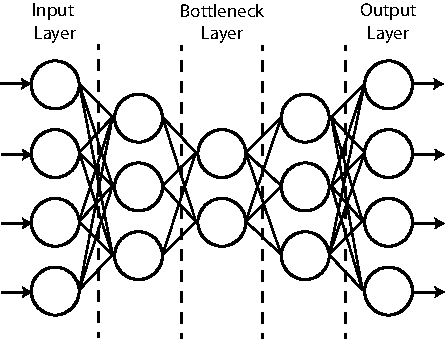
\includegraphics{resources/simple_autoencoder.pdf}
            \caption{Diagram representing a very basic autoencoder. It can be seen the the hidden layers introduces fewer and fewer nodes from the input layer. In doing so creates a bottle neck for the input data.}
            \label{fig:autoencoder}
        \end{figure}
    \subsubsection{Particle Swarm Optimisation}
        \hspace*{0pt}\hfill \textit{An Vo}\\
        
    \subsubsection{Distortions and Noise in Optical Communication System}
        \hspace*{0pt}\hfill \textit{An Vo}\\
        
        An optical communication channel is comprised of a transmitter, receiver and the optical fibre connecting the two together. In order to simulate this communication channel, the mathematical representation of the signal at each stage of the channel needs to be established. The signal that enters the optical fibre is described by its electrical field of the EM field, known as its optical field and is expressed mathematically in the time domain as: 
    
        \begin{equation}
            \label{eqn:optical_field_time}
            A(t, z) = |A(t,z)|e^{j\phi(t,z)}
        \end{equation}
        where $z$ is the distance along the fibre and $t$ is the time. $A(t,z)$ is a phasor incorporating the optical amplitude $|A(t,z)|$ and optical phase $\phi(t,z)$.
        \\
        
        The signal suffers from chromatic dispersion as it traverses through the optical fibre, resulting in different frequency components of the signal being delayed by different amounts. For simulation simplicity, this effect will be simulated in the frequency domain due to a linear time delay vs frequency and can be expressed by the following mathematical expression:
        
        \begin{equation}
            \label{eqn:optical_field_freq}
            A(\omega,L) = A(\omega,0)e^{j\frac{1}{2}\beta_z\omega^2L}
        \end{equation}
        where $\omega$ is angular frequency, $\beta_z$ is the group velocity dispersion and $L$ is the fibre length.
        \\
        
        At the receiver, photo-detection is carried out by using the proportional relationship between the output voltage and power of the signal which in turn is proportional to the square of the magnitude of the optical field, resulting in the following mathematical expression.
        
        \begin{equation}
            \label{eqn:squared_law_detection}
            V_{out}(t) = |A(t,L)|^2
        \end{equation}
        where $A(t,L)$ is the inverse Fourier transform of \autoref{eqn:optical_field_freq}.
        \\
        
        To complete the mathematical representation of the signal through an optical channel, the receiver noise is applied to the photo-detected signal. This is in the form of white Gaussian noise (randomly generated voltages $\Delta V(t)$, which are generated with a normal distribution) which is added to both the model shot noise and the thermal noise. This voltage waveform is then the representation of the signal after it leaves the receiver.
        \\
        
        The transmitting and receiving end as well as the channel itself need to be simulated as a channel model. The neural networks will most likely be implemented using the TensorFlow package with python. The python programming language was chosen for quick prototyping purposes as well as compatibility with TensorFlow. TensorFlow allows for quick experimentation and configuration of different neural network architectures. The above proposed model would be treated as a black box between the transmitting and receiving neural network. 
    
\subsection{Progress to Date}

    \subsubsection{Familiarization with tensorflow}
    % tf/leras layer subclassing, model subclassing, IQ autoencoder
    
    \begin{figure}[H]
		\centering
		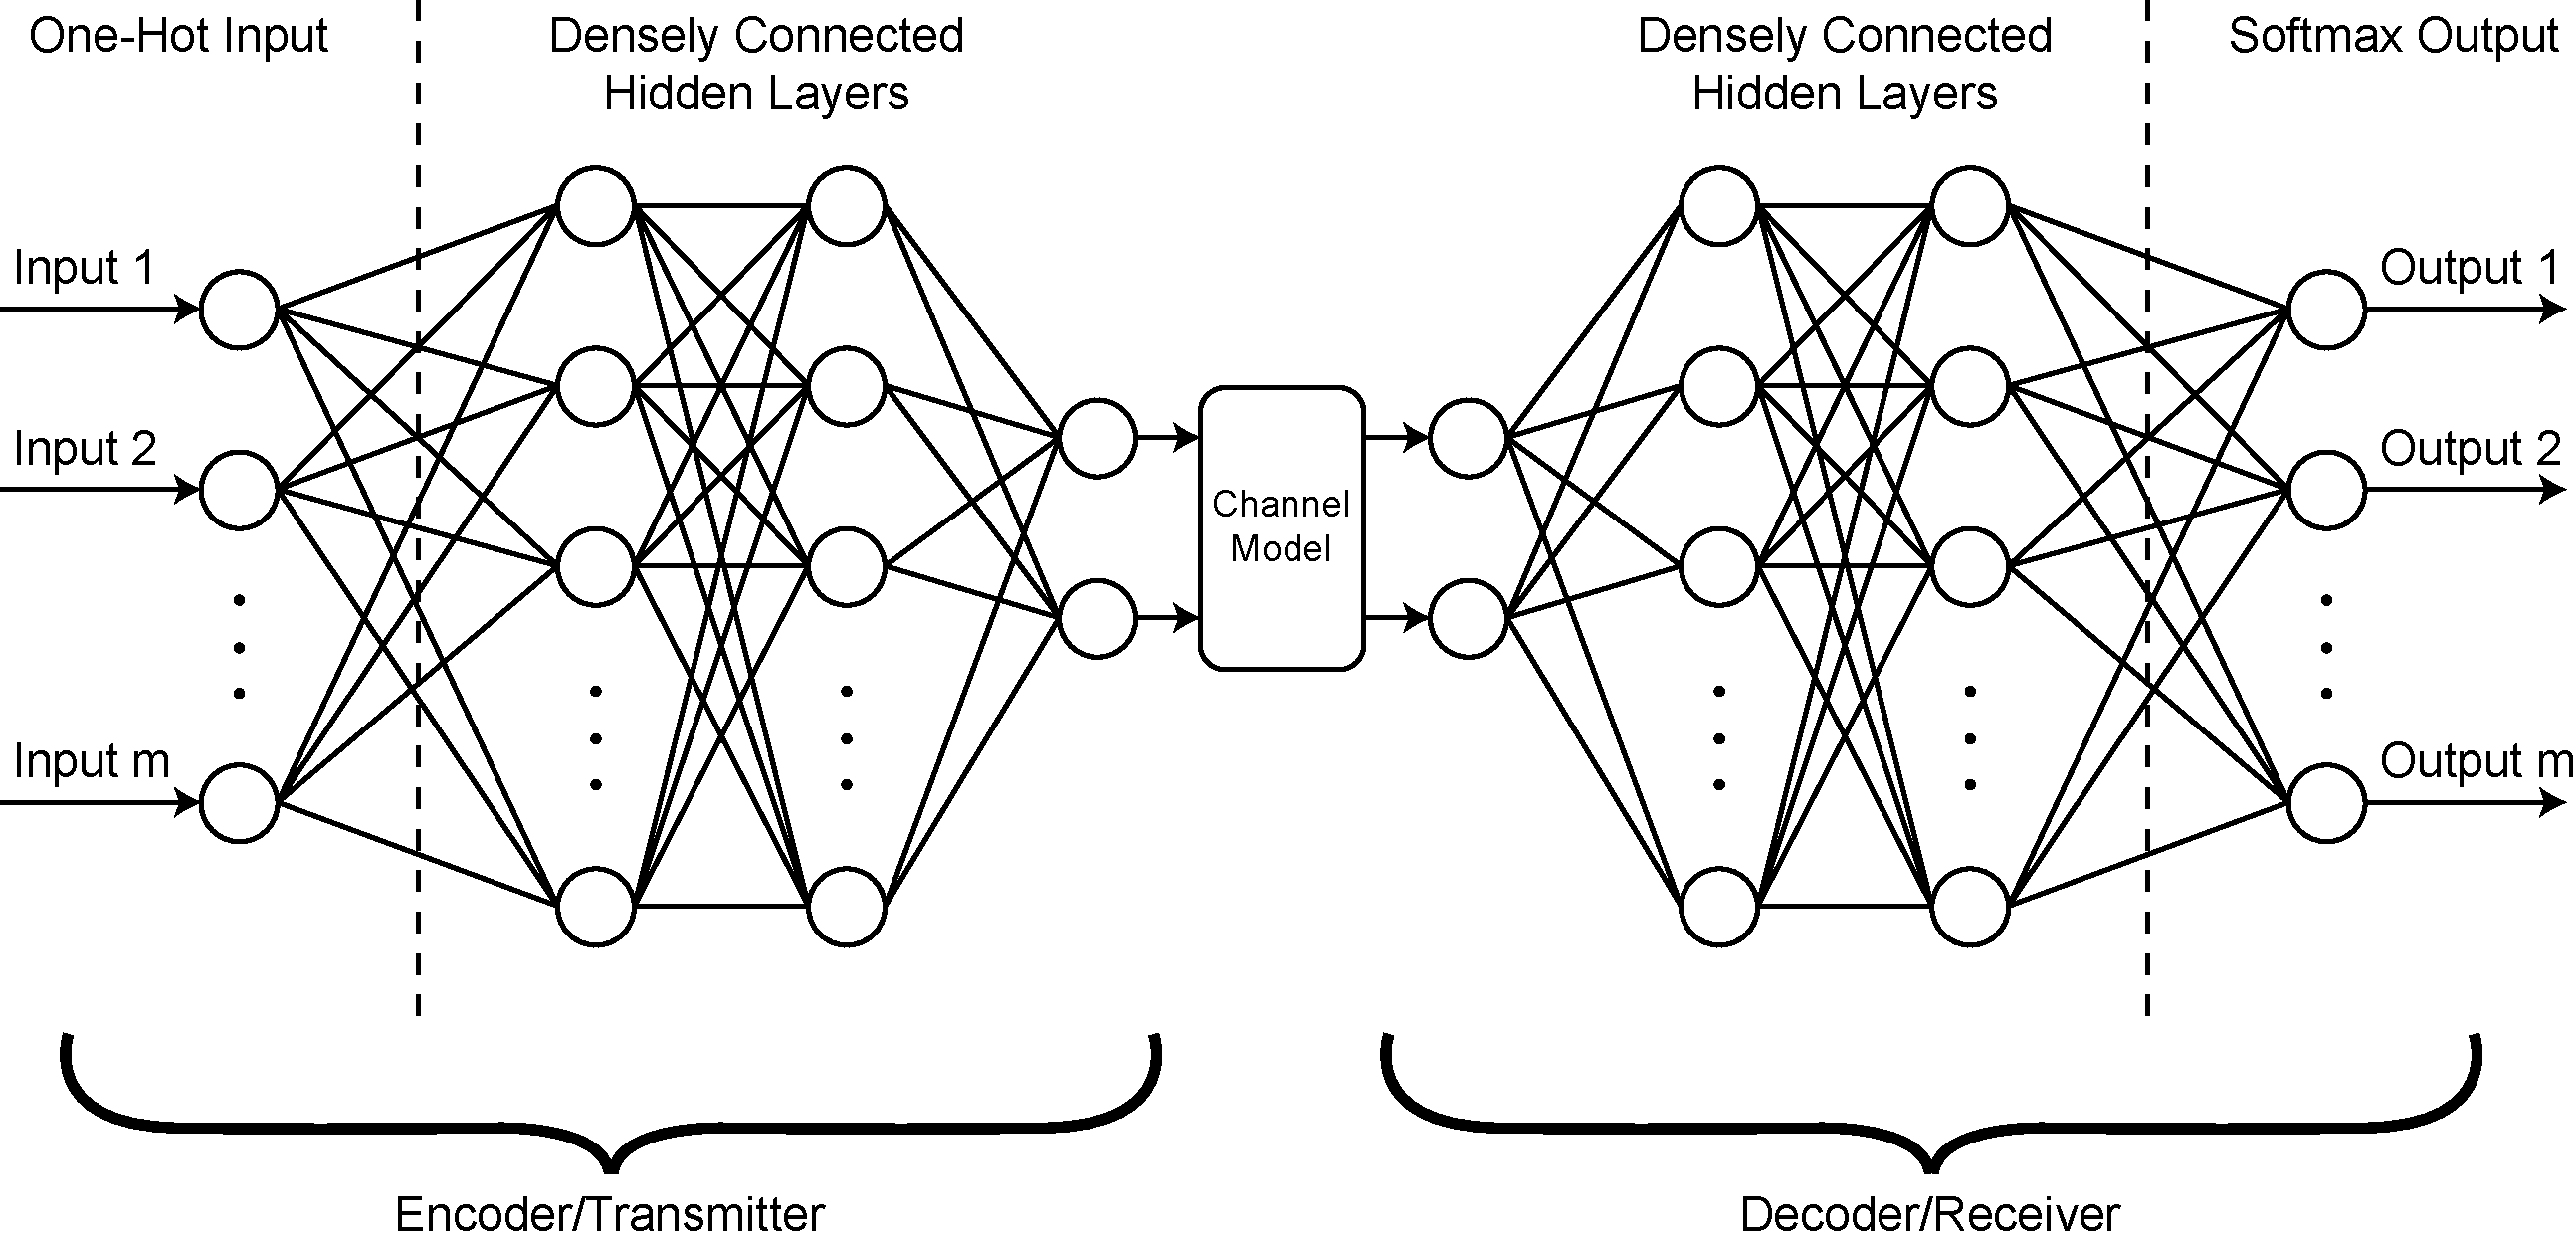
\includegraphics[scale=0.35]{iq_autoencoder_diagram.pdf}
		\caption{Diagram representing the neural network that was implemented. The encoding and decoding sections are also labelled. The one-hot input layer is of size $m=\log_2 N$ where $N$ is the number of bits encoded per message. The softmax output layer produces a probability vector conveying the probability that the received signal corresponds to any of the messages.}
		\label{fig:iq_autoencoder_diagram}	
	\end{figure}
    
    \subsubsection{Optical Channel Model}
    \hspace*{0pt}\hfill \textit{Tharmetharan Balendran}\\
    
    The optical channel model consists of 3 main components: The application of chromatic dispersion, the squared law detection as well as the addition of Gaussian noise. The chromatic dispersion was applied by taking the fast Fourier transform (FFT) of the incoming signal and applying a phase shift that is proportional to the frequency as shown by \autoref{eqn:optical_field_freq}. Following this, the signal is transformed back to time domain using an inverse fast Fourier transform (IFFT). After the chromatic dispersion is applied, the detection of the signal by a photodiode is simulated. This is represented by \autoref{eqn:squared_law_detection}. The absolute value of the signal is taken and squared to produce the receiver output. Following this, additive white Gaussian noise (AWGN) was applied to simulate noise arising from the receiver components (amplifiers, thermal noise, etc.) The figures in \autoref{fig:optical_channel_model_signals} show the distortion being applied for a simple on off keying (OOK) modulation scheme with rectangular pulse shapes. 
    
    \begin{figure}[H]
		\begin{subfigure}{0.5\textwidth}
			\centering
			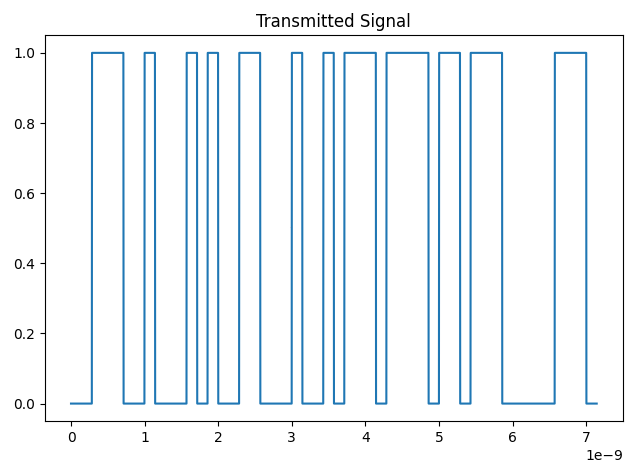
\includegraphics[scale=0.5]{transmitted_signal.png}
			\caption{Transmitted signal using a On-Off-Keying (OOK) modulation for simplicity.}
			\label{fig:transmitted_signal}	
		\end{subfigure}
		\begin{subfigure}{0.5\textwidth}
			\centering
			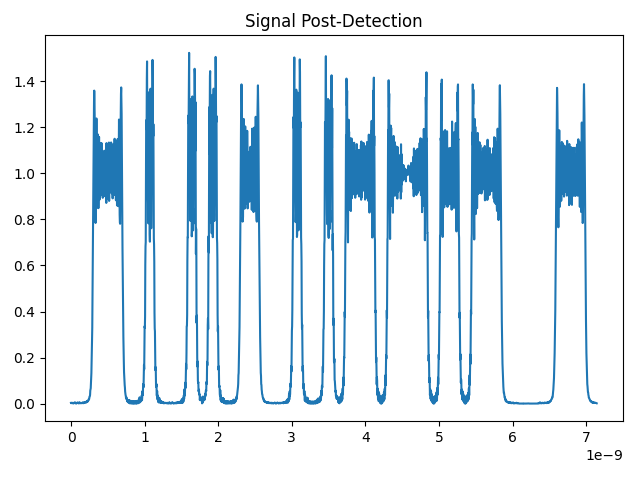
\includegraphics[scale=0.5]{signal_post_detection.png}
			\caption{Received signal after all distortions of the signal have been applied.}
			\label{fig:signal_post_detection}	
		\end{subfigure}
		\caption{Plots showing the distortion of the transmitted signal over an optical fibre of length 10km with a group velocity dispersion of -21.7 $ps^2/km$. The sample rate was set to 336 GHz while the bit rate was set to 7 GHz}
		\label{fig:optical_channel_model_signals}
	\end{figure}
    
    \subsubsection{Implementation of DSP and Signal Analysis Techniques}
    % pulse shaping, eye diagram, BER vs SNR plots,
    \textbf{Pulse Shaping} \hspace*{0pt}\hfill \textit{Tharmetharan Balendran}\\
    
        Different pulse shapes were implemented to enable the transmission of pulse amplitude modulation (PAM) signals with efficient bandwidth usage. The pulse shapes to choose from in the simulation are: rectangular, raised cosine and root raised cosine. These were implemented by convolving their impulse functions with the time domain representation of the signal. The raised cosine filter pulse shape can be seen in the eye diagram in \autoref{fig:eye_diagram}.
        \\
    
    \textbf{BER vs SNR} \hspace*{0pt}\hfill \textit{Oliver Jaison}\\
    
        We were facing problems in measuring the performance of the model and the channel so code was implemented to generate a graph of BER against Noise and BER (Bit Error Rate) against SNR (Signal to Noise Ratio) shown in \autoref{fig:ber_vs_snr}. This way we could now measure the performance of the model and the channel.
        \\
        
    \textbf{Eye Diagrams} \hspace*{0pt}\hfill \textit{Oliver Jaison}\\
    
    Upon observing strange results from the BER vs SNR figures we implemented code to generate an eye diagram for the transmitted signal so that the quality of the signal could be analysed. An example of this can be seen in \autoref{fig:eye_diagram} .
    
    \begin{figure}[H]
		\begin{subfigure}{0.5\textwidth}
			\centering
			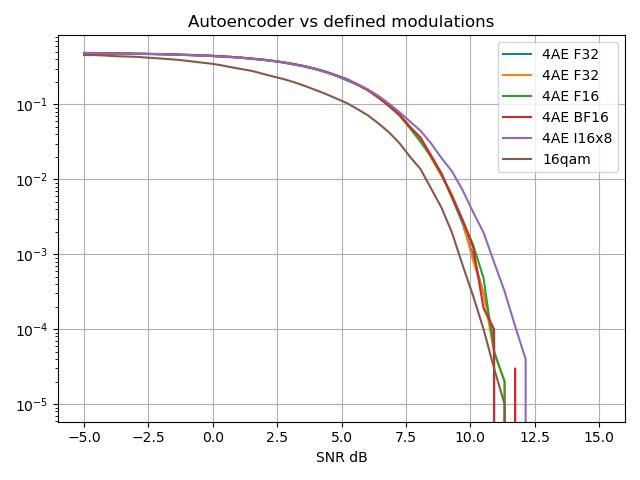
\includegraphics[width=\textwidth]{post-train-quan.jpg}
			\caption{This figure shows a graph of BER against SNR for different modulation methods.}
			\label{fig:ber_vs_snr}	
		\end{subfigure}
		\begin{subfigure}{0.5\textwidth}
			\centering
			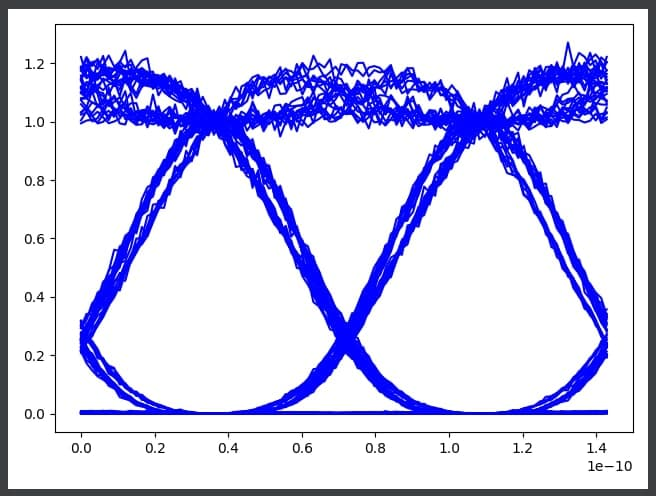
\includegraphics[width=\textwidth]{model_eye_diagram.jpg}
			\caption{This is an example eye diagram of a received signal of a 2PAM modulated signal with a raised cosine pulse shape.}
			\label{fig:eye_diagram}	
		\end{subfigure}
		\caption{Plots of different performance measuring metrics used to identify any faults in the channel models or modulation techniques.}
		\label{fig:optical_channel_model_signals}
	\end{figure}
    
    \subsubsection{Replication of Neural Network discussed by B. Karanov et al. \autocite{8433895}}
    \hspace*{0pt}\hfill \textit{Tharmetharan Balendran}\\
    
    The neural network configuration discussed in this paper demonstrated promising results and would be a good place to start. The paper discussed a simple feed-forward neural network autoencoder. The encoding neural network acts as a modulator and produces encoded symbols for each message at the bottleneck layer. The bottleneck output is passed through a channel model to simulate transmission distortions and then passed into the decoding neural network that acts as the demodulator. On the encoding neural network, $N$ identical neural networks encode $N$ consecutive messages into $N$ consecutive symbols each consisting of $n$ samples. These symbols are then serialized to form a single stream of $n\times N$ samples. This ensures that inter-symbol interference (ISI) can be modelled by considering neighbouring symbols. At the decoding neural network, the central symbol is extracted and demodulated. The complete architecture of the autoencoder can be seen in \autoref{fig:end_to_end_autoencoder_diagram}.
    
    \begin{figure}[H]
		\centering
		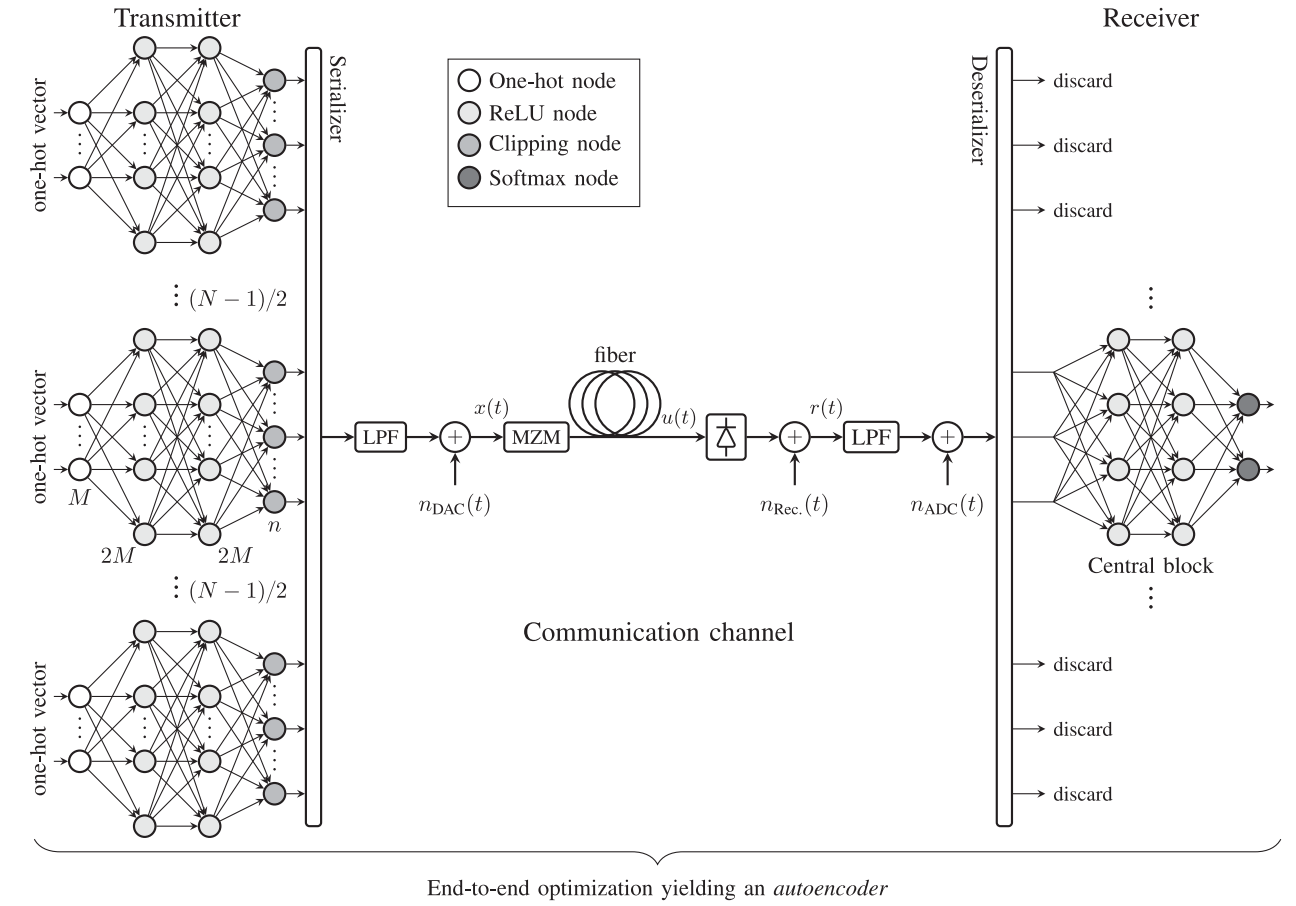
\includegraphics[width=0.9\textwidth]{end_to_end_autoencoder_diagram.png}
		\caption{The diagram taken from \autocite{8433895} depicting the overall configuration to enable learning of symbols.}
		\label{fig:end_to_end_autoencoder_diagram}	
	\end{figure}
    
    A similar implementation of the autoencoder was configured using the tensorflow package in python. In this implementation the simulation of the Mach-Zehnder modulator (MZM) was left out to simplify the channel model. As the MZM operates linearly for small amplitudes, this assumption would not harm the accuracy of the simulation greatly. To enable this, the optical channel model had to be re-developed to be compatible with tensorflow's tensor datatype. This was achieved by utilizing tensorflow functions for fast Fourier transforms (FFT) as well as tensor multiplication. The optical channel was implemented as a tensorflow layer and can therefore be placed in-between the encoder and decoder.
    \\

    Symbol mapping similar to those discussed in \autocite{8433895} was achieved. A complete mapping of messages onto symbols can be seen in \autoref{app:learnt_symbol_mapping}. No specific mapping of bits onto symbols was enforced meaning that no assessment as to the potential BER of the system can be made. From testing the autoencoder with appropriate noise a symbol error rate of around $1\times10^{-2}$ was observed. The simulation parameters are given in \autoref{tab:simulation_parameters}.
    \\
    \begin{table}[H]
        \centering
        \begin{tabular}{ll}
            \textbf{Parameter}                              & \textbf{Value}            \\ \hline
            Sampling Frequency ($f_{s}$)                    & $336\;GHz$                 \\
            Message Cardinality ($M$)                       & $32$                      \\
            Samples per Symbol ($n$)                        & $24$                      \\
            Messages per Block ($N$)                        & $9$                       \\
            Dispersion Factor ($\beta$)                     & $-21.7\;ps^{2}km^{-1}$     \\
            Fiber Length ($L$)                              & $50\;km$                   \\
            Receiver Noise stddev (\sigma_{rx}$)            & $0.01$                    \\
            Quantization Noise stddev (\sigma_{rx}$)        & $0.002$
        \end{tabular}
        \caption{Table of simulation parameters used when learning symbol mapping using the end-to-end autoencoder.}
        \label{tab:simulation_parameters}
    \end{table}
    
    As the chromatic dispersion results in ISI, an encoder/decoder that is able to consider previously received/transmitted symbols should outperform one that solely considers one symbol at a time. To simulate this, long-short-term-memory (LSTM) layers were implemented at the transmitting and receiving neural networks. These will still need further tuning to produce acceptable results but should outperform the feed-forward neural network architecture.
    
    \subsubsection{Application of Particle Swarm Optimisation} \hspace*{0pt}\hfill \textit{An Vo}\\
    \subsubsection{Neural Network Hyperparamter Optimisation} \hspace*{0pt}\hfill \textit{An Vo}\\
    
    \subsubsection{Choice of FPGA and DAC for Hardware Implementation}
    
    \subsubsection{Implementation of simple Neural Network in a HDL}